\documentclass{article}


\usepackage[letterpaper,margin=0.75in]{geometry}
\usepackage[utf8]{inputenc}

\usepackage{graphicx}

\usepackage{hyperref}
\hypersetup{
    colorlinks=true,
    linkcolor=blue,
    filecolor=blue,      
    urlcolor=blue,
    citecolor=blue,
}

\usepackage{biblatex}
\addbibresource{sample.bib}

\title{ME 556 Project Report Template}
\author{Eric Homer\\ ME 556 Project Report \\ Brigham Young University}
\date{\today}

\begin{document}

\maketitle
\begin{abstract}
Replace the text here with a short overview of your paper. This section has instructions about the general organizational structure used in this document and some comments about writing using \LaTeX{}.

If you have questions about the best practices to follow when writing a paper like this, I recommend reading documents about the \href{https://en.wikipedia.org/wiki/IMRAD}{IMRaD} organizational structure. The BYU Mechanical Engineering Department also has documentation about how to write the various sections of IMRaD in this \href{http://me.byu.edu/resources}{BYU ME Writing Materials} link. In particular, I expect your figures and tables to follow the instructions listed in the BYU writing link.

You \textbf{must} use the sections illustrated in this document, but you do not have to use \LaTeX{}. If you do wish to use \LaTeX{} and you are new to this, I recommend using \href{https://www.overleaf.com}{Overleaf}. Overleaf has a great guide to \LaTeX{} and tips on formatting in their \href{https://www.overleaf.com/learn}{Documentation}. To use this in Overleaf, create a new project, upload these files, and then recompile whenever you want to see the latest PDF of your manuscript. In the text below I have listed examples of how to use lists, equations, figures, and tables. New paragraphs can be obtained by having an extra line in between lines of text.



\end{abstract}



\section{Introduction}
\label{sec:intro}
Replace the text in this section with the text of your paper. This section currently lists information about project outcomes, examples of past projects, and assignments associated with this project.

\subsection{Project outcomes}

\begin{enumerate}
    \item Chance to learn try out a modeling technique on a problem of interest to you
    \item Learn how to validate a modeling technique to ensure meaningful results and understand the limitations of the selected technique
    \item Learn to interpret results in the context of your modeling approach and its limitations as well as that of the literature to which the work contributes

\end{enumerate}

\subsection{Examples}
Here is a brief list of past projects:
\begin{itemize}
    \item Atomistic simulations of grain boundary mobility
    \item Atomistic simulations of deformation in a polycrystal
    \item Finite element - KMC simulations of deformation in a metallic glass
    \item Phase stability of a material using cluster expansion
    \item Potts model simulation of microstructure evolution
    \item Machine learning using a grain boundary metric of similarity
    \item Molecular modeling of MEMS spring
\end{itemize}

\subsection{Assignments}
The following assignments will be due on dates listed on \href{https://learningsuite.byu.edu}{Learning Suite}.

\begin{enumerate}
    \item Initial overview of problem (recommended that you turn in a draft of your introduction section)
    \begin{itemize}
        \item Need to meet with me
        \item Keep project conservative
        \item Can be new to you but already published in the literature, IF a complete description is NOT published
    \end{itemize}
    
    \item Planned methods (recommended that you turn in a draft of your methods section)
    \item Initial results (recommended that you turn in a draft of your validation, results, and, if possible, discussion sections)
    \item Presentation
    \item Final report using the overall layout listed in this file (minus this descriptive text in the introduction and other examples of how to add a figure and table.)


\end{enumerate}

\noindent Note: You may receive extra credit if your report is of sufficient quality to be submitted to a journal. But this is a significant investment of time and effort, only 1 person has done it in 3 semesters.


\section{Background}
\subsection{Scientific Principle}
feel free to change this subsection title


Here is an example of a book reference \cite{Pumphrey:1975dl} and an article reference \cite{Wolf:1992we}. Note that the two look the same here, but different in the bibliography at the end of the document.


\subsection{Modeling Approaches}
feel free to change this subsection title

\section{Methods}
\label{sec:methods}
The following is an example equation for the free energy of a shape memory alloy.

\begin{equation}
    d\psi = -S dT  - \varepsilon d\sigma
    \label{eqn:freeenergy_TS}
\end{equation}

\noindent In Equation \ref{eqn:freeenergy_TS}, $S$ is entropy, $T$ is temperature, $\varepsilon$ is strain, and $\sigma$ is stress. Note the \\ref{} command used to reference a specific equation.


\section{Model Validation}
\label{sec:validation}
In this section, Table \ref{tab:GBdata} is given as an example of how to format a table in \LaTeX{}.

\begin{table}
\centering
\caption{Information about the $\left[1\,0\,0\right]$ disorientation axis grain boundaries studied in this work.}   
   \begin{tabular}{ c c c}
   \hline
   CSL $\Sigma$ Number & Disorientation Angle [$^{\circ}$] & Number of GBs \\
   \hline
   85a & 8.80 & 52 \\
25a & 16.26 & 59 \\
13a & 22.62 & 80 \\
17a & 28.07 & 72 \\
  5 & 36.87 & 66 \\
29a & 43.60 & 53 \\
   \hline
   
   \end{tabular}
\label{tab:GBdata}   
\end{table}


\section{Results}
\label{sec:results}

In this section, Figure \ref{fig:Rodrigues} is given as an example of how to format a figure in \LaTeX{}.

\begin{figure}[htb]
    \centering
    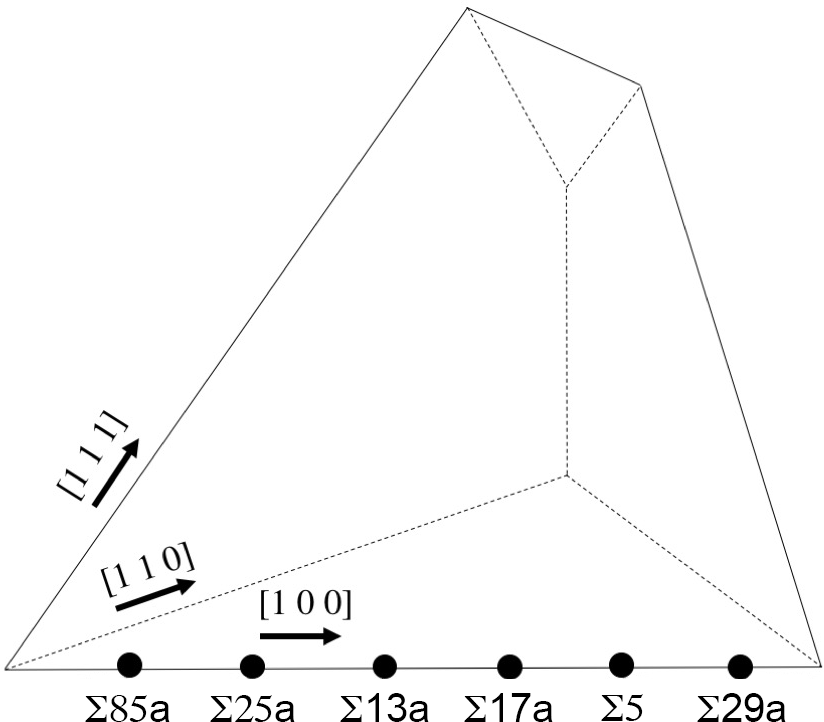
\includegraphics[width=0.5\columnwidth]{Rodrigues}
    \caption{The six CSL misorientations from Table \ref{tab:GBdata} plotted along the $\left[1\,0\,0\right]$ disorientation axis represented in the Rodrigues fundamental zone for cubic-cubic misorientations.}
    \label{fig:Rodrigues}
\end{figure}

\section {Discussion}
\label{sec:discussion}


\section{Conclusions}
\label{conclusions}

In addition to your conclusions, include lessons learned and future improvements that could be implemented.




\printbibliography

\end{document}